%%%%%%%%%%%%%%%%%%%%%%%%%%%%%%%%%%%%%%%%%
% Short Sectioned Assignment
% LaTeX Template
% Version 1.0 (5/5/12)
%
% This template has been downloaded from:
% http://www.LaTeXTemplates.com
%
% Original author:
% Frits Wenneker (http://www.howtotex.com)
%
% License:
% CC BY-NC-SA 3.0 (http://creativecommons.org/licenses/by-nc-sa/3.0/)
%
%%%%%%%%%%%%%%%%%%%%%%%%%%%%%%%%%%%%%%%%%

%----------------------------------------------------------------------------------------
%	PACKAGES AND OTHER DOCUMENT CONFIGURATIONS
%----------------------------------------------------------------------------------------

\documentclass[paper=a4, fontsize=11pt]{scrartcl} % A4 paper and 11pt font size

\usepackage[T1]{fontenc} % Use 8-bit encoding that has 256 glyphs
\usepackage{fourier} % Use the Adobe Utopia font for the document - comment this line to return to the LaTeX default
\usepackage[english]{babel} % English language/hyphenation
\usepackage{amsmath,amsfonts,amsthm} % Math packages

\usepackage{graphicx}

\usepackage{sectsty} % Allows customizing section commands
\allsectionsfont{\centering \normalfont\scshape} % Make all sections centered, the default font and small caps

\usepackage[procnames]{listings}

\usepackage{fancyhdr} % Custom headers and footers
\pagestyle{fancyplain} % Makes all pages in the document conform to the custom headers and footers
\fancyhead{} % No page header - if you want one, create it in the same way as the footers below
\fancyfoot[L]{} % Empty left footer
\fancyfoot[C]{} % Empty center footer
\fancyfoot[R]{\thepage} % Page numbering for right footer
\renewcommand{\headrulewidth}{0pt} % Remove header underlines
\renewcommand{\footrulewidth}{0pt} % Remove footer underlines
\setlength{\headheight}{13.6pt} % Customize the height of the header
\usepackage{float}

\numberwithin{equation}{section} % Number equations within sections (i.e. 1.1, 1.2, 2.1, 2.2 instead of 1, 2, 3, 4)
\numberwithin{figure}{section} % Number figures within sections (i.e. 1.1, 1.2, 2.1, 2.2 instead of 1, 2, 3, 4)
\numberwithin{table}{section} % Number tables within sections (i.e. 1.1, 1.2, 2.1, 2.2 instead of 1, 2, 3, 4)

\setlength\parindent{0pt} % Removes all indentation from paragraphs - comment this line for an assignment with lots of text

%----------------------------------------------------------------------------------------
%	TITLE SECTION
%----------------------------------------------------------------------------------------

\newcommand{\horrule}[1]{\rule{\linewidth}{#1}} % Create horizontal rule command with 1 argument of height

\title{	
\normalfont \normalsize 
\textsc{BRSU} \\ [25pt] % Your university, school and/or department name(s)
\horrule{0.5pt} \\[0.4cm] % Thin top horizontal rule
\huge Neural Networks\\Assignment 9 \\ % The assignment title
\horrule{2pt} \\[0.5cm] % Thick bottom horizontal rule
}

\author{Bastian Lang} % Your name

\date{\normalsize\today} % Today's date or a custom date

\begin{document}

\maketitle % Print the title

\newpage



\section{Exercise 2}

\subsection{Task}
The graphs below represent three different one-dimensional classification
(dichotomization) tasks (along a sketched x-axis, dash means "no data point")(figure \ref{fig_ex2}.
What is the lowest-order polynomial decision function that can correctly classify the
given data? Black dots denote class 1 with target function value y1 = +1 and white dots
depict class 2 with targets y2 = -1. What are the decision boundaries?
\begin{figure}[H]
	\centering
  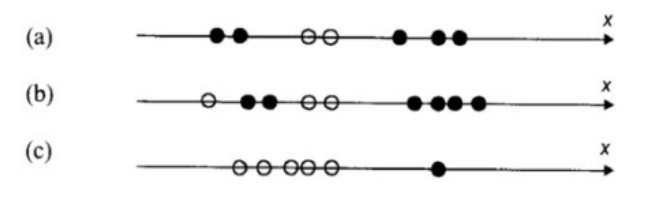
\includegraphics[width=0.8\textwidth]{exercise2.png}
	\caption{}
	\label{fig_ex2}
\end{figure}

If you wanted to classify the data sets (a), (b), (c) using SVM's with Gaussian basis
functions, how many hidden layer neurons would you need for each problem?

\subsection{Solution}
The order depends on the number of turning points. For one turning point a polynomial of order 2 is needed.\\
(a) The lowest order polynomial would be 2 (parabola).\\
(b) The lowest order polynomial would be 3.\\
(c) The lowest order polynomial would be 1 (line).\\

The number of hidden layer neurons equals the order of the polynomial needed -1.

\section{Exercise 3}
\subsection{Results}
For the linear kernel the decision boundary obviously is a line, which works good if the separation is 0, but the worse the more the two figures are intermixed.\vspace{5mm}

RBF works well for all figures but the one were the figures are overlapping.\vspace{5mm}

Using polynomial kernel with default degree of 3 I would have expected a better fit, but even low separation results in some errors, the overleaping figures do look similar to the linear kernel version.\\ Looking at the data increasing the degree should not help because degree 3 should be sufficient. But my laptop is not able to come up with a result within 10 minutes for higher degree.\\
Maybe just repeating with degree 3 several times will yield better results.
\subsection{Output}
\subsubsection{Sampled Pairs}
\begin{figure}[H]
	\centering
  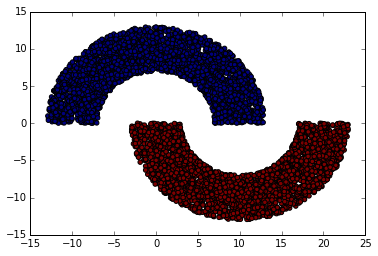
\includegraphics[width=0.8\textwidth]{samples_1.png}
	\caption{Test data with vertical separation = 0}
	\label{fig_s1}
\end{figure}
\begin{figure}[H]
	\centering
  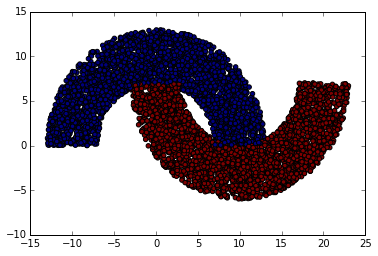
\includegraphics[width=0.8\textwidth]{samples_2.png}
	\caption{Test data with vertical separation = -1/2 * (radius - 1/2*width)}
	\label{fig_s2}
\end{figure}
\begin{figure}[H]
	\centering
  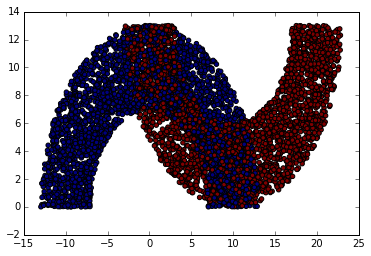
\includegraphics[width=0.8\textwidth]{samples_3.png}
	\caption{Test data with vertical separation = - radius of inner half circle}
	\label{fig_s3}
\end{figure}
\begin{figure}[H]
	\centering
  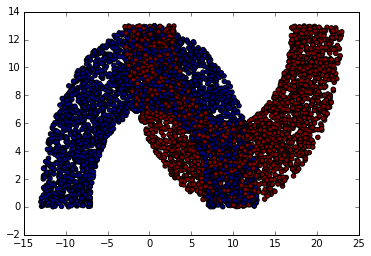
\includegraphics[width=0.8\textwidth]{samples_4.png}
	\caption{Test data with vertical separation = - radius of outer half circle}
	\label{fig_s4}
\end{figure}

\subsubsection{Linear Kernel}
\begin{figure}[H]
	\centering
  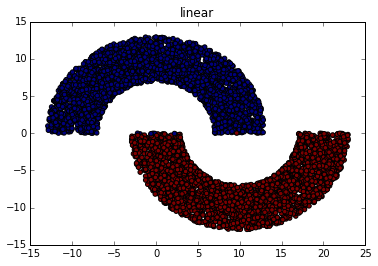
\includegraphics[width=0.8\textwidth]{linear_1.png}
	\caption{Classified test pairs with vertical separation = 0 using linear kernel}
	\label{fig_l1}
\end{figure}
\begin{figure}[H]
	\centering
  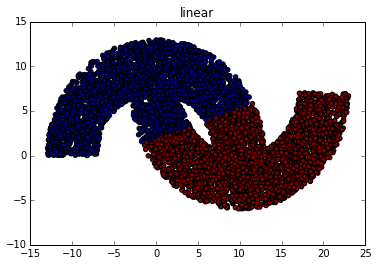
\includegraphics[width=0.8\textwidth]{linear_2.png}
	\caption{Classified test pairs with vertical separation = -1/2 * (radius - 1/2*width) using linear kernel}
	\label{fig_l2}
\end{figure}
\begin{figure}[H]
	\centering
  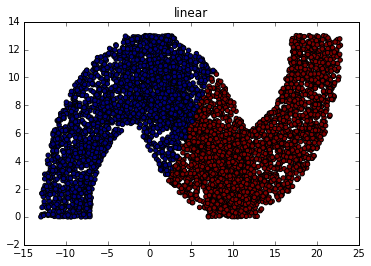
\includegraphics[width=0.8\textwidth]{linear_3.png}
	\caption{Classified test pairs with vertical separation = - radius of inner half circle using linear kernel}
	\label{fig_l3}
\end{figure}
\begin{figure}[H]
	\centering
  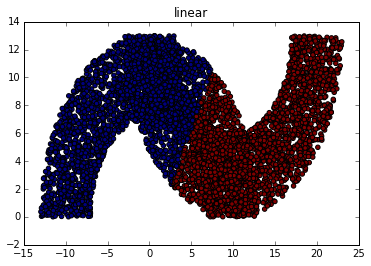
\includegraphics[width=0.8\textwidth]{linear_4.png}
	\caption{Classified test pairs with vertical separation = - radius of outer half circle using linear kernel}
	\label{fig_l4}
\end{figure}

\subsubsection{RBF}
\begin{figure}[H]
	\centering
  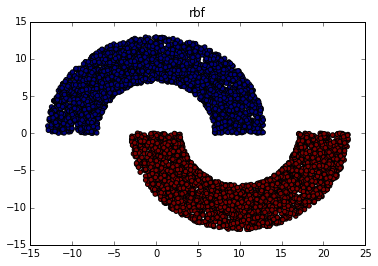
\includegraphics[width=0.8\textwidth]{rbf_1.png}
	\caption{Classified test pairs with vertical separation = 0 using rbf kernel}
	\label{fig_rbf1}
\end{figure}
\begin{figure}[H]
	\centering
  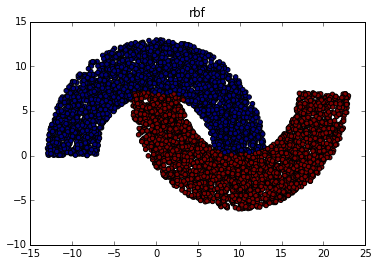
\includegraphics[width=0.8\textwidth]{rbf_2.png}
	\caption{Classified test pairs with vertical separation = -1/2 * (radius - 1/2*width) using rbf kernel}
	\label{fig_rbf2}
\end{figure}
\begin{figure}[H]
	\centering
  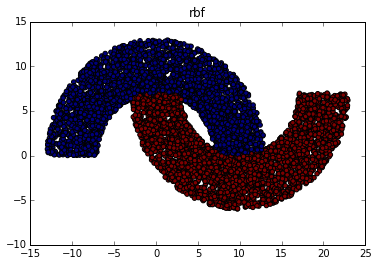
\includegraphics[width=0.8\textwidth]{rbf_3.png}
	\caption{Classified test pairs with vertical separation = - radius of inner half circle using rbf kernel}
	\label{fig_rbf3}
\end{figure}
\begin{figure}[H]
	\centering
  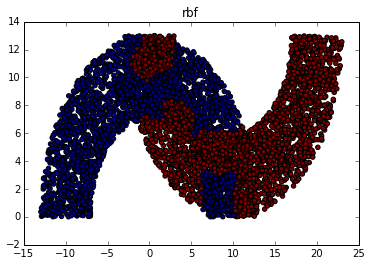
\includegraphics[width=0.8\textwidth]{rbf_4.png}
	\caption{Classified test pairs with vertical separation = - radius of outer half circle using rbf kernel}
	\label{fig_rbf4}
\end{figure}

\subsubsection{Polynomial}
\begin{figure}[H]
	\centering
  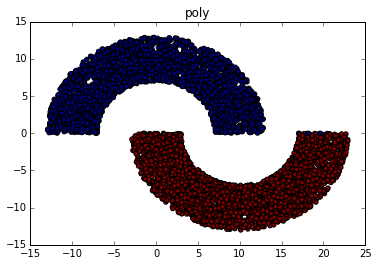
\includegraphics[width=0.8\textwidth]{poly_1.png}
	\caption{Classified test pairs with vertical separation = 0 using polynomial kernel}
	\label{fig_poly1}
\end{figure}
\begin{figure}[H]
	\centering
  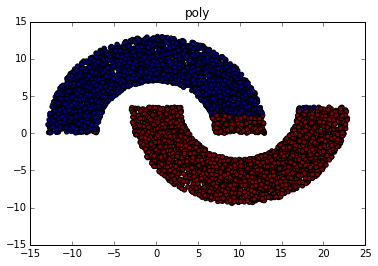
\includegraphics[width=0.8\textwidth]{poly_2.png}
	\caption{Classified test pairs with vertical separation = -1/2 * (radius - 1/2*width) using polynomial kernel}
	\label{fig_poly2}
\end{figure}
\begin{figure}[H]
	\centering
  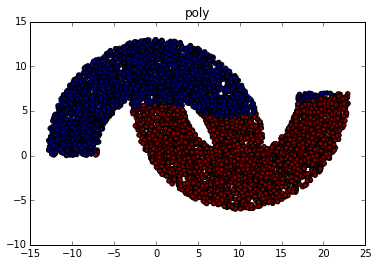
\includegraphics[width=0.8\textwidth]{poly_3.png}
	\caption{Classified test pairs with vertical separation = - radius of inner half circle using polynomial kernel}
	\label{fig_poly3}
\end{figure}
\begin{figure}[H]
	\centering
  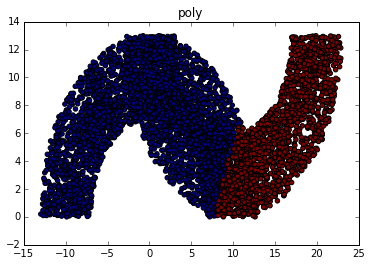
\includegraphics[width=0.8\textwidth]{poly_4.png}
	\caption{Classified test pairs with vertical separation = - radius of outer half circle using polynomial kernel}
	\label{fig_poly4}
\end{figure}

\subsubsection{Code}
\begin{lstlisting}
# -*- coding: utf-8 -*-
"""
Created on Thu Dec  3 22:36:41 2015

@author: bastian
"""

import random
import numpy as np
from matplotlib import pyplot as plt
from sklearn.cluster import KMeans
from sklearn.svm import *

RADIUS = 10
WIDTH = 6
VERTICAL_SEPARATION = 0

# TODO: SVM is supervised -> assign labels according to part of upper or lower half moon

def sample_upper_halfmoon(radius, width):
    distance = random.random() * width + radius - 0.5 * width
    angle = random.random() * 180
    angle = np.radians(angle)
    x = np.cos(angle) * distance
    y = np.sin(angle) * distance
    return [x,y]
    
def sample_lower_halfmoon(radius, width, vertical_separation):
    distance = random.random() * width + radius - 0.5 * width
    angle = random.random() * 180 + 180
    angle = np.radians(angle)
    x = np.cos(angle) * distance + radius
    y = np.sin(angle) * distance - vertical_separation
    return [x,y]

    
def sample_pair(radius, width, vertical_separation):
    a = sample_upper_halfmoon(radius, width)
    b = sample_lower_halfmoon(radius, width, vertical_separation)
    return a,b
    
def plot_points_with_specified_separaration(vertical_separation):
    training_samples_x = []
    training_samples_y = []
    training_class = []
    for i in range(1000):
        a,b = sample_pair(RADIUS,WIDTH, vertical_separation)
        training_samples_x.append(a[0])
        training_samples_x.append(b[0])
        training_samples_y.append(a[1])
        training_samples_y.append(b[1])
        training_class.append(-1)
        training_class.append(1)
        
    test_samples_x = []
    test_samples_y = []
    test_class = []
    for i in range(3000):
        a,b = sample_pair(RADIUS,WIDTH, vertical_separation)
        test_samples_x.append(a[0])
        test_samples_x.append(b[0])
        test_samples_y.append(a[1])
        test_samples_y.append(b[1])
        test_class.append(-1)
        test_class.append(1)
        
    figure = plt.figure()
    ax = figure.add_subplot(111)
    ax.scatter(test_samples_x, test_samples_y, c=np.array(test_class).astype(np.float))
    return  training_samples_x, training_samples_y, training_class, test_samples_x, test_samples_y, test_class



def fit_and_predict(samples, kernel_type):
    training = np.array([samples[0], samples[1]], dtype='float64').T
    clf = SVC(kernel=kernel_type).fit(training, np.array(samples[2], dtype='float64'))
    prediction = clf.predict(np.array([samples[3],samples[4]], dtype='float64').T)
    fig1 = plt.figure()
    plt.title(kernel_type)
    ax1 = fig1.add_subplot(111)
    ax1.scatter(samples[3],samples[4], c=prediction.astype(np.float))

set1=plot_points_with_specified_separaration(0)
set2=plot_points_with_specified_separaration((-0.5) * (RADIUS-0.5*WIDTH))
set3=plot_points_with_specified_separaration((-1) * (RADIUS-0.5*WIDTH))
set4=plot_points_with_specified_separaration((-1) * (RADIUS+0.5*WIDTH))

fit_and_predict(set1, 'linear')
fit_and_predict(set2, 'linear')
fit_and_predict(set3, 'linear')
fit_and_predict(set4, 'linear')

fit_and_predict(set1, 'rbf')
fit_and_predict(set2, 'rbf')
fit_and_predict(set3, 'rbf')
fit_and_predict(set4, 'rbf')

fit_and_predict(set1, 'poly')
fit_and_predict(set2, 'poly')
fit_and_predict(set3, 'poly')
fit_and_predict(set4, 'poly')

fit_and_predict(set1, 'sigmoid')
fit_and_predict(set2, 'sigmoid')
fit_and_predict(set3, 'sigmoid')
fit_and_predict(set4, 'sigmoid')


\end{lstlisting}

\end{document}